\documentclass[11pt,a4paper]{article}

\usepackage{amsmath,amssymb}
\usepackage{graphicx}
\usepackage{epsfig}

\begin{document}

\title{How to put figures into LaTeX}
\author{Hans Krister Frisk}
\maketitle

\begin{abstract}
 I made two figures in Mathematica and now it is time to get
 them into the text.
\end{abstract}



\section{Two figures}

Important that eps-file lies in same folder as this tex-document.
\begin{figure}[tbph]
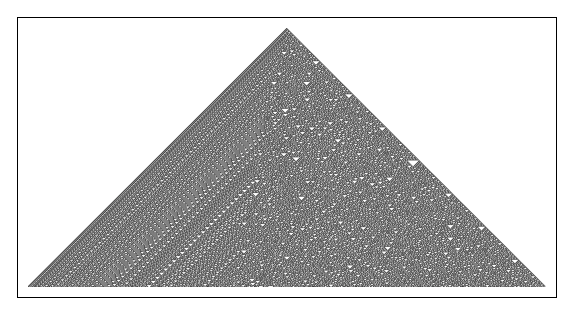
\epsfig{file=plot1.eps}
\caption{ This figure illustrates three geometrical concepts.
Point, circle and line.}
\end{figure}

There it came! Now we have a look at the second figure.
  
\begin{figure}[tbph]
\epsfig{file=plot4.eps}
\caption{ The curve is $\sin x$ and the line $\frac{x}{2}$. To solve
the equation $\sin x = \frac{x}{2}$ a numerical method is needed. 
}
\end{figure}
 
To get it on paper you use Build in TeXnicCenter. If you have eps-files
use LaTeX $\rightarrow$ PS $\rightarrow$ PDF in the box. Figure 2 came out below this text.
Disturbed by Out sign in plots? You can cut them in Mathematica. Do you want frame, axes labels etc
for your plot? No problem, see Plot command in Mathematica. You write Plot, mark it with mouse and select
Find Selected Function in the help menu.



\end{document}
